\section{Compilación local} 
\label{sec:local}

Si utilizas Overleaf con una cuenta gratuita es muy posible que excedas el límite de tiempo para compilar. Nuestra recomendación es que tu tutor cree el proyecto correspondiente a tu TFG y te lo comparta como colaborador con permiso de escritura.  Pero también puedes compilarlo localmente en tu propio ordenador instalando algo de software. Como ha sido una preocupación recurrente, hemos cambiado la plantilla para que sea más fácil de compilar en Microsoft Windows.

\begin{enumerate}
\item Instala \href{https://www.texstudio.org/}{TexStudio}. Es un editor de \LaTeX{} no tan sencillo como Overleaf pero mucho más amigable que editar los archivos en un editor de texto normal.
\item Instala \href{https://miktex.org/download}{MikTeX}. Si marcas la opción \emph{Install missing packages on the fly} los paquetes de \LaTeX{} se instalarán automáticamente, que resulta muy conveniente.
\item Si usas Windows instala \href{https://strawberryperl.com/}{Strawberry Perl}. Es necesario para utilizar la orden \emph{Latexmk} en la compilación.
\item Instala \href{https://python.org}{Python}. Lo necesitarás si usas el entorno \textbf{minted} para colorear trozos de código. A la hora de instalar Python no olvides marcar la casilla para añadir Python a la variable de entorno \texttt{Path}.
\end{enumerate}

\subsection{Configurar el entorno}

\begin{enumerate}
\item Abre la aplicación \emph{MikTeX Console} e instala las fuentes de la plantilla. Para ello pincha en \emph{Packages} y añade los paquetes \texttt{stix}, \texttt{stix2-type1}, \texttt{stix2-otf}, \texttt{arial} y \texttt{noto}.
\item Añade la carpeta que contiene \path{perl.exe} a la variable de entorno \texttt{Path}.  Si instalaste Strawberry Perl en el lugar por omisión debes añadir \path{C:\Strawberry\perl\bin}.
\item Elimina el alias de ejecución de Python de Windows.  Para ello pulsa la tecla de Windows y escribe \texttt{alias}, selecciona \emph{Administrar alias de ejecución de aplicaciones}. Asegúrate que el alias del \emph{Instalador de aplicaciones} no está activado para \texttt{python.exe} y \texttt{python3.exe}.
\end{enumerate}

Comprueba que todo está correctamente configurado.  Para ello abre una ventana de órdenes (PowerShell o Símbolo de sistema) y teclea \texttt{perl -v} y posteriormente \texttt{python -V}. Ambas órdenes deberían ejecutarse sin error y mostrar las versiones de Perl y Python respectivamente. Por último ejecuta \texttt{pip install Pygments} que instalará el software de coloreado de código.

\subsection{Configurar TeXStudio}

Entra en \emph{Opciones $\rightarrow$ Configurar TeXStudio} y configura la sección \emph{Compilar} como se muestra en la \autoref{fig:cfg-compilar-texstudio}. El compilador por defecto debe ser \textbf{Latexmk} y la herramienta bibliográfica debe ser \textbf{Biber}.

\begin{figure}
    \centering
    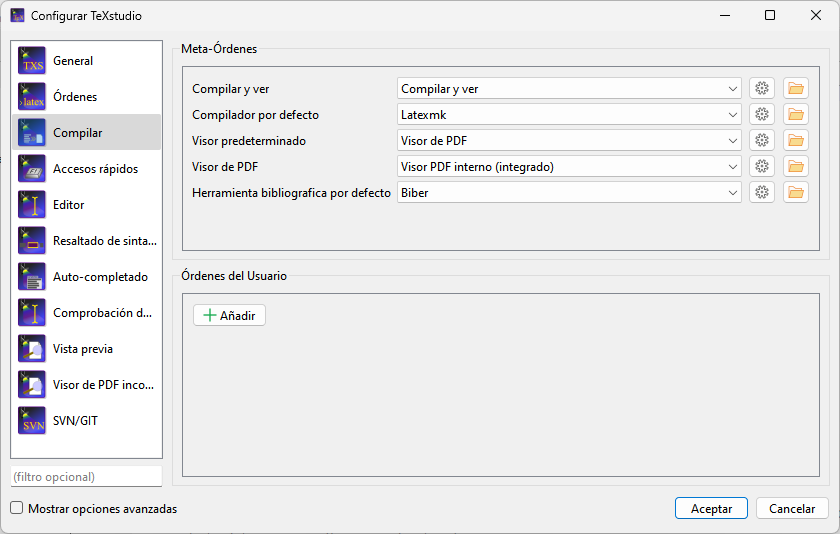
\includegraphics[width=.7\textwidth]{fig/cfg-texstudio-compilar.png}
    \caption{Configuración de la compilación en TeXStudio}
    \label{fig:cfg-compilar-texstudio}
\end{figure}

Entra en la sección \emph{Órdenes} y modifica las opciones de \emph{Latexmk} como muestra la~\autoref{fig:cfg-ordenes-texstudio}. La opción \texttt{-pdf} debe ser sustituida por \texttt{-lualatex -shell-escape}.

\begin{figure}
    \centering
    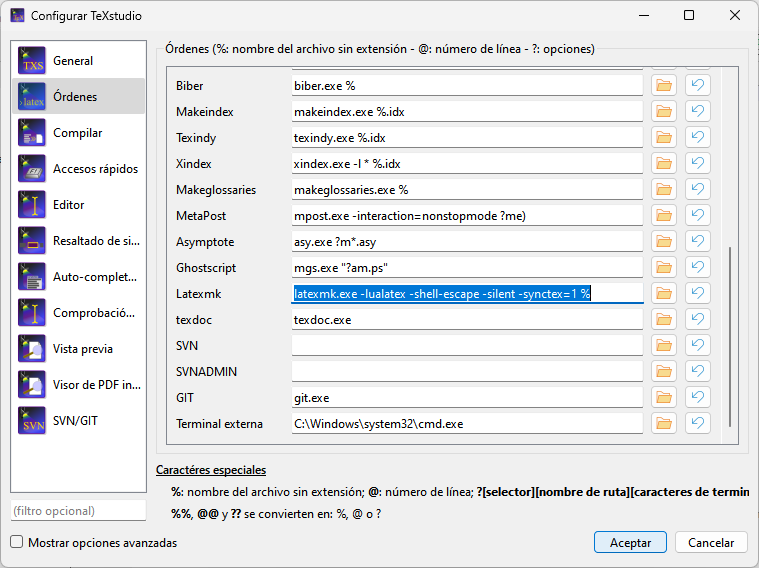
\includegraphics[width=.7\textwidth]{fig/cfg-texstudio-ordenes.png}
    \caption{Configuración de la orden \emph{Latexmk} en TeXStudio}
    \label{fig:cfg-ordenes-texstudio}
\end{figure}

Una vez configurado, para compilar el documento solo hay que pulsar en el botón \textbf{Compilar} 
\includegraphics{texstudio-compilar.png}. Para previsualizar el resultado hay que pulsar sobre el botón \textbf{Visualizar} 
\includegraphics{texstudio-preview.png}.